\documentclass{article}

\usepackage[utf8]{inputenc}
\usepackage[spanish]{babel}
\usepackage{fullpage}
\usepackage{hyperref}
\usepackage{graphicx}
\usepackage{mathtools}
\usepackage{amsmath}
\usepackage{sidecap}
\usepackage{listings}
\usepackage{color}
\usepackage{setspace}

\title{Informe de tesis de licenciatura}
\author{Ionatan Perez}
\date{\today}




\begin{document}

\spacing{1.5}



% Cosas del formateo para la inclusion del codigo
\definecolor{dkgreen}{rgb}{0,0.6,0}
\definecolor{gray}{rgb}{0.5,0.5,0.5}
\definecolor{mauve}{rgb}{0.58,0,0.82}
\renewcommand{\lstlistingname}{Código}
\lstset{frame=tb,
  language=Java,
  aboveskip=3mm,
  belowskip=3mm,
  showstringspaces=false,
  columns=flexible,
  basicstyle={\small\ttfamily},
  numbers=none,
  numberstyle=\tiny\color{gray},
  keywordstyle=\color{blue},
  commentstyle=\color{dkgreen},
  stringstyle=\color{mauve},
  breaklines=true,
  breakatwhitespace=true,
  tabsize=3
}




\maketitle

\clearpage 

\tableofcontents  %lo ponemos para trabajo largos que necesiten indice
\clearpage

\section{Introducción}

    Los mecanismos y dispositivos de sustitución sensorial (SSD) son técnicas en las cuales los estimulo generados en nuestro entorno y que normalmente son percibido a través de un dado sentido son reemplazados por otro estimulo (pero que codifica información equivalente) de manera que pueda ser percibido a través de un sentido sensorial alternativo. Típicamente estas técnicas son utilizadas por personas que carecen de alguno de los sentidos para poder percibir lo que de otra manera no podrían. Ejemplos cotidianos de estas técnicas son por ejemplo el bastón que suelen usar las personas ciegas, las marcas y guías en baldosas, el código braille, los timbres que encienden luces, las escalas cromáticas aptas para daltónicos, etc. 
    
    En particular, dentro de los problemas biológicos de percepción, el problema de la ceguera es un problema que conlleva limitaciones muy importantes para las personas que la sufren y que afecta a cerca de diez millones de personas en el mundo \cite{NroCiegos}. Como paliativo a dicha situación existen diferentes técnicas (algunas de muy baja complejidad, pero funcionalidad limitada) para sustituir sensorialmente los estímulos, como puede ser un bastón que al tacto permita reconocer obstáculos. Otras técnicas, mucho mas complejas y en actual desarrollo, apuntan a restituir la capacidad de visión mediante implantes que estimulen artificialmente al sistema nervioso\cite{Implantes1,Implantes2}, pero actualmente se encuentran en un estado muy temprano de desarrollo, solo sirven en casos específicos, poseen poca resolución y son muy invasivas \cite{Implantes3,Implantes4}. 
    
    Alternativamente a las técnicas que buscan restituir la visión en personas ciegas, están las técnicas que sustituyen los estímulos, estos estímulos pueden ser reemplazados por estímulos táctiles o bien auditivos. La representación táctil de los estímulos visuales comparte la propiedad intrínseca de ser percibida en un sistema de coordenadas bidimencional (la piel y la retina ambos poseen sensores distribuidos en una superficie). Los trabajos pioneros en este técnica fueron realizados por Paul Bach-y-Rita \cite{Tactil1} quien diseñó un dispositivo que sujeto en la espalda de las personas podía reproducir imágenes filmadas por una cámara. Sin embargo la baja resolución de este dispositivo (20x20 pixeles), junto a su tamaño hicieron que sea poco practico. En posteriores trabajos \cite{Tactil2} se reemplazó el dispositivo por uno colocado en la legua (que posee una sensibilidad muy alta) donde además se reemplazó el mecanismo de estímulo por uno de pequeñas descargas eléctricas. Este trabajo solucionó en buena parte el problema de la portabilidad del dispositivo (que media 3cmx3cm con 12x12 pixeles), pero sin embargo su capacidad de distinguir objetos sigue siendo reducida \cite{Tactil3}, comparable (sin entrenamiento) a 20/860 \footnote{Esta manera de indicar la capacidad visual de una persona representa cuan lejos tiene que estar (medido en pies si el numerador es 20) de dos puntos para distinguirlos en relación a una persona con visión plena. Se suele considerar a una persona con problemas de ceguera cuando su capacidad esta por debajo de 20/200}. Estudios \cite{Tactil4} muestran que con entrenamiento los sujetos pueden mejorar en cu capacidad de percepción, sin embargo hay una limitación básica en la resolución que permite este dispositivos que esta dado por la separación espacial de los electrodos y la capacidad de la lengua de distinguirlos. 
    
    \begin{figure}
        \center
        \includegraphics[width=0.8\textwidth]{Imagenes/Voice2.png}
        \caption{Dispositivo de sustitución sensorial vOICe y ejemplo de representación de las imagenes a través de dicho dispositivo.}
        \label{fig:Voice2}
    \end{figure}
    
    \begin{figure}
        \center
        \includegraphics[width=0.8\textwidth]{Imagenes/ImagenVoice1.png}
        \caption{Perdida de resolución al utilizar una tecnología tipo vOICe, se compara la imagen original con la imagen pixelada luego del procesamiento y la resolución real observada en sujetos. \url{http://dx.doi.org/10.1371/journal.pone.0033136}}
        \label{fig:Voice1}
    \end{figure}
    
    \begin{figure}
        \center
        \includegraphics[width=0.7\textwidth]{Imagenes/Voice3.png}
        \caption{Ejemplo del sonido correspondiente a imágenes pertenecientes a diferentes categorías y la capacidad del distinguirlas en sujetos que fueron entrenados durante periodos de tiempo prolongado en la tecnología vOICe. \url{http://dx.doi.org/10.1016/j.neuron.2012.08.026}}
        \label{fig:Voice3}
    \end{figure}
    
    
    El otro mecanismo por el cual se puede realizar sustitución sensorial es transformando el estimulo visual en un estímulo sonoro. El primer prototipo de esta tecnología (denominada vOICe) fue desarrollado en 1992 \cite{Voice1} como un dispositivo portátil, de bajo costo y de resolución mayor a las alcanzadas por los métodos de sustitución táctil (ver figura \ref{fig:Voice1}). Con el tiempo se fueron desarrollando versiones mejores, de mayor resolución y adaptadas a las tecnologías mas modernas (ver figura \ref{fig:Voice2}).
    
    La tecnología vOICe (\url{https://www.seeingwithsound.com/}), a diferencia de la sustitución sensorial táctil presenta la libertad de elegir que parámetros del sonido se eligen para representar los parámetros que usualmente se observan con la vista. A priori hay una amplia libertad en la representación si utilizan efectos sonoros complejos, sin embargo, recurriendo a las características básica del sonido hay tres grados de libertad a la hora de crear un sonido: el tono o frecuencia, el volumen y la duración. Estas tres características son las que utiliza el vOICe para representar la información visual (codificada en escala de grises). El vOICe toma una imagen, la pixela, y representa la coordenada vertical de cada pixel en la frecuencia, la coordenada horizontal en el tiempo (o duración del pixel) y la intensidad (o brillo) del pixel en el volumen o intensidad del sonido. En otras palabras lo que hace es interpretar cada columna de la imagen como una antitransformada de fourier del sonido a generar. 
    
    A partir de esta concepción de sustitución sensorial, el vOICe se fue desarrollando sobre diferentes plataformas tecnológicas siendo hoy una aplicación disponible en diversas plataformas, incluyendo PCs, celulares, y otros dispositivos que sean capaces de grabar imágenes y reproducir sonidos. Además cuenta con herramientas integradas de utilidad para personas ciegas como ser comandos por vos, filtros del la imagen a procesar por color, geolocalizacion, etc. La version para celulares pude consultarse en \url{https://play.google.com/store/apps/details?id=vOICe.vOICe} y un manual para realizar el entrenamiento adecuado para su uso en \url {https://www.seeingwithsound.com/manual/The_vOICe_Training_Manual.htm} 
    
    En paralelo al desarrollo de la tecnología vOICe como aplicación, se realizaron otras pruebas e investigaciones, algunas sobre variantes en la representación sonora, como ser el caso de la denominada PSVA \cite{VoiceVariante1} que difiere del vOICe en que la escala vertical esta discretizada no en función de la resolución como numero de pixeles, sino respetando saltos que difieran en notas fijas, además posee una región de mayor resolución en la zona central de la imagen, simulando el funcionamiento del ojo. Otra variante es el denominado SmartSight que filtra y agrupa secciones de la imagen antes de realizar una representación sonora en forma de notas musicales \cite{VoiceVariantes2, VoiceVariantes3}. También sobre la base de codificar diferentes aspectos en términos de propiedades sonoras mas complejas, se esta desarrollando una versión similar el vOICe denominada EyeMusic que codifica en términos de notas la altura de los pixeles, pero utilizando diferentes instrumentos para representar diferentes colores \cite{VoiceVariantes4}.
    
    Por otro lado a partir del imágenes y mediciones de actividad cerebral y de entrenamiento se han realizado estudios acerca del funcionamiento subyacente al mecanismo de sustitución sensorial. Hay estudios que muestran que en el caso de personas ciegas de nacimiento se activas zonas típicas de procesamiento de la información para el canal sensorial utilizado, mientras que en personas que perdieron la visión siendo adultos se activan zonas del procesamiento de imágenes (frente a un mismo estimulo), o que la modulación de la actividad cerebral difiere entre personas que perdieron la vista a edad temprana y personas que simplemente reciben el estimulo con la vista tapada \cite{VoiceSubyacente1,VoiceSubyacente3}. También hay estudios que muestran que con entrenamiento los sujetos aprenden a reconocer patrones fijos e incluso pueden transferir el aprendizaje entre figuras similares \cite{VoiceSubyacente2}. Por otro lado estudios sobre la tecnología vOICe muestran que los sujetos son capaces de entrenar e integrar la percepción en tareas de reconocimiento de geometría espacial, siendo capaces de ubicar y señalar posicionamiento de objetos en un entorno 3D donde pueden cambiar el punto de vista de la cámara con la que observan los estímulos \cite{VoiceSubyacente4}
    
    Los trabajos previos sobre la tecnología vOICe muestran que los sujetos entrenados (que pueden ser tanto ciegos como videntes\cite{VoiceEntrenamiento1}) pueden aprender a distinguir entre categorías imágenes complejas \cite{VoiceEntrenamiento2} (como los que se observan en la figura \ref{fig:Voice3}), nosotros en nuestro trabajo intentamos sobre la base de un sistema de representación equivalente estudiar la capacidad no de interpretar figuras complejas, sino sencillas, pero en términos de categorías geométricas. 
    
    La idea detrás de la propuesta fue que, si bien a la hora de interactuar con entornos complejos es importante que el sistema de sustitución sensorial permita representar de forma equivalente información compleja, muchas actividades no requieren interactuar con estímulos complejos. Muchas veces los estímulos o bien son intrínsecamente sencillos (por ejemplo los iconos y contornos en la navegación dentro de una computadora) o bien se puede preprocesar la imagen para extraer con algoritmos las información mas relevante antes de realizar la sustitución sensorial. Por otro lado, estudiar la capacidad de detectar conceptos geométricos abstractos podría permitir inspeccionar, dentro de la compleja tarea de reconocer patrones, saber que aspectos son mas difíciles de identificar, cuales mas fáciles, y de que depende la dificultad a la hora de interpretar los sonidos. También teníamos como objetivo tratar de identificar en que procesos del aprendizaje se podía observar efectos de transferencia (tanto dentro de una categoría como en orientaciones y otras trasformaciones de simetría)
    
    Con ese objetivo en mente fue que nos propusimos realizar experimentos en los cuales se presentara a sujetos videntes estímulos sonoros codificados según la lógica del vOICe en pos de observar cual era la capacidad de los sujetos de distinguir los aspectos geométricos en estos estímulos. 


\section{Desarrollo Metodológico}

\subsection{Panorama general del trabajo realizado}

    Poder realizar los experimentos propuestos conllevo una larga lista de desafíos, elecciones y problemas técnicos a resolver, en muchos casos interrelacionados y con desconocimiento de la dificultad que representaría cada elección a priori. Cualquiera de los diseños experimentales que nos propusiéramos tenía que consistir en la presentación de estímulos sonoros al usuario (o sujeto experimental) que debían ser respondido con alguna elección. Posteriormente correlacionando los estímulos presentados con las respuestas se podría evaluar la capacidad de percepción del sujeto. Pero la elección de estímulos, la secuencia en la cual presentarlos, el modo en que interactuaría el sujeto con el experimento, las condiciones de entorno en que sería realizado, y las preguntas especificas que buscábamos responder eran en un principio cuestiones abiertas.
    
    Algunas cuestiones que si estaban definidas eran que en un principio todos los sujetos serian videntes porque experimentos previos de entrenamiento \cite{VoiceEntrenamiento3} indicaban que los videntes presentan capacidades similares de aprender la representación que las personas ciegas, y conseguir sujetos tanto como interactuar con ellos durante el procedimiento experimental es muchísimo más fácil si los sujetos son videntes. Eventualmente una vez obtenidos resultados se podrían contrastar y validar en personas no videntes. 
        
    Los desafíos que tuvimos que encarar a lo largo de todo el trabajo de la tesis probablemente puedan englobarse en unas pocas categorías, sin embargo la interacción y avance en cada una de ellas no fue lineal ni independiente por lo que su raconto a lo largo de este informe no va a respetar un orden estrictamente temporal sino más bien conceptual. Agrupando en categorías las dificultad que tuvimos que ir superando se pueden resumir en:
    
    \begin{itemize}
        \item Generar los estímulos. Diseñar la creación en forma sistemática y paramétrica de conjuntos de estímulos que permitieran probar las hipótesis de trabajo. 
        \item Adaptar, caracterizar y testear un algoritmo compatible con el resto del código que transformara los estímulos en su correspondiente representación sonora, y que respondiera a la lógica del vOICe. 
        \item Diseñar los experimentos que quisiéramos realizas y en función de ello generar los estímulos y niveles (instrucciones para crear un conjuntos de trials (o pruebas) consecutivos con las especificaciones necesarias).
        \item Diseñar la lógica de ejecución en tiempo real mediante la cual el experimento adapta los estímulos a mostrar en función de las respuestas de los usuarios (esto fue particularmente importante en los últimos experimentos)
        \item Diseñar una aplicación que fuera capaz de interpretar e integrar en una interfaz con el usuario toda la información relacionada a los estímulos y niveles creados manejando en tiempo real la elección de estímulos y parámetros según correspondiera, así como el correcto registro de múltiples indicadores que permitieran luego reconstruir por completo lo realizado por el sujeto experimental. 
        \item Construir un servidor que permitiera almacenar los datos en forma remota y que sirviera para realizar luego consultas a la hora de procesar la información en busca de resultados.
        \item Procesar los datos registrados para validar las hipótesis del diseño experimental y proponer adaptaciones o cambios en al mismo. 
    \end{itemize}
    
    En términos temporales el primer desafío que nos propusimos fue hacer un experimento en el que pudiéramos saber si los usuarios eran capaces de distinguir figuras geométricas, para ello pensamos en segmentos paralelos o no paralelos, ángulos rectos o no rectos y cuadriláteros cuadrados o no cuadrados (esto últimos son una combinación de las dos categorías anteriores y permitirían evaluar procesos de transferencia). El resultado (luego de muchas pruebas preliminares, ajustes, calibraciones y horas de programación) fue satisfactorio en tanto los sujetos eran capaces de interpretar al menos en términos muy básicos las figuras geométricas (generadas medio al azar) y distinguir entre grandes categorías o ejemplos muy diferentes. Esto no era obvio que fuera a suceder ya que los trabajos previos requerían decenas de horas de entrenamiento mientras que nuestros experimentos tenían que involucrar mucho menos tiempo de entrenamiento. Sin embargo surgieron dos problemas a la hora de pensar en un proceso de entrenamiento o medición mas cuidadoso. En primer lugar resultó evidente que la representación sonora es fuertemente no invariante frente a rotaciones, es clave la orientación de los segmentos que conforman las figuras a la hora de establecer la dificultad de interpretarlos y esta dependencia no la teníamos caracterizada. Por otro lado no teníamos ningún parámetro de la dificultad para cada estímulo en particular, por lo tanto no teníamos manera de armar un conjunto de estímulos que de alguna manera pudieran distinguir la capacidad en la zona de parámetros donde no saturara la medición como muy fácil o muy difícil. 
    
    Cabe aclarar que todas las mediciones de esta primer etapa fueron realizadas en forma esporádica y sin llevar un protocolo unificado que permitiera extraer conclusiones o resultados numéricamente validos. Por esto, cuando ya contábamos con una versión de la aplicación bastante funcional y una noción de las dificultades encontradas decidimos realizar un primer experimento piloto en el cual intentaríamos medir la dependencia con la orientación en la dificultad de distinguir entre categorías. Este experimento implico definir y ajustar varias cuestiones relacionadas al diseño experimental y los algoritmos necesarios para implementarlo. El primero y mas importante fue que en lugar de distinguir entre categorías para estímulos aleatorios necesitábamos caracterizar la capacidad de los sujetos en una tarea especifica y para eso queríamos realizar un experimento tipo Quest donde midiéramos el umbral de detección en función de la orientación. Este cambio requería por un lado generar secuencias de estímulos similares que variaran en una única dimensión o parámetro de manera de poder fluctuar dicho parámetro hasta encontrar el punto donde el usuario pasara de distinguir el estimulo a no distinguirlo. Por otro lado requería adaptar la lógica de funcionamiento de la aplicación y de los niveles para que pudieran ajustar la dificultad del estimulo mostrado en tiempo real en lugar de repetir una secuencia preestablecida. Además en la realización de este experimento pusimos a prueba todas las dificultades inherentes a la logística de realizar un experimento en laboratorio siguiendo un protocolo formal.
    
    Los resultados de este experimento mostraron que efectivamente la dependencia de la dificultad con la orientación existía y era muy marcada, pero también mostraron que había una enorme variabilidad intersujeto por lo cual no tenia sentido establecer la dificultad de un estimulo como parámetro intrínseco del estímulo. Por otro lado en este experimento descartamos evaluar los cuadriláteros por carecer las características geométricas necesarias. 
    
    A esta altura la idea de medir y entrenar a los sujetos (como habíamos pensado en un principio) con estímulos genéricos y comunes a todos los sujetos resultaba inviable. También resultaba inviable la idea de hacer un experimento masivo (en celulares o internet) ya que para poder evaluar cualquier característica era necesario una calibración previa que demanda una disponibilidad de tiempo y continuidad difícil de conseguir en un experimento a distancia. Por ello ideamos un último experimento en condiciones controladas de laboratorio donde lo que buscaríamos observar era si el entrenamiento en alguna condición especifica producía una mejora en la performance del sujeto durante y luego del entrenamiento, y si se observa una transferencia de dicha mejora entre las condiciones evaluadas. Para eso diseñamos un protocolo en el cual medimos la performance inicial de los sujetos, luego a algunos sujetos los entrenamos (dándoles feedback acerca de sus respuestas) en la detección de ángulos, a otros en la detección de paralelas y a otros no los entrenamos. Por ultimo volvimos a medir la performance de todos los sujetos con la intención de poder comparar el efecto del entrenamiento. 
    
    Como parte de los cambios realizados en el protocolo, mejoramos el mecanismo de medición del umbral respecto al experimento anterior (cambiando la lógica de generación de estímulos, y el algoritmo dinámico para ajustar la dificultad porque el largo de los experimentos resultaba un limitante), elegimos un conjunto de configuraciones o niveles con un alto grado de simetría con el objetivo de distinguir si la posible transferencia dependía de algunos de estos invariantes, y seleccionamos las configuraciones donde los sujetos mostraban peor performance inicial con el objetivo de tener un mayor rango donde medir los efectos de la mejora. Como se puede observar en los resultados detallados más adelante los resultados de este experimento no dieron todo lo bien que esperábamos. La principal razón por la cual no pudimos observar resultados acordes a lo buscado la atribuimos al bajo numero de sujetos que conseguimos que participaran del experimento, lo cual invalida cualquier medición estadísticamente sólida y al hecho de que el proceso de entrenamiento parece ser mas bien de carácter cualitativo y no cualitativo, es decir que cuando los sujetos entienden lo que tienen que hacer presentan una mejora, pero que dicha mejora luego no se repite en el tiempo al menos en los tiempos y longitudes de entrenamiento realizado. 
    
\subsection{El proceso de creación de estímulos} \label{seccion:SVG}
    
    Desarrollar el proceso de creación de estímulos implicó dos desafíos, por un lado disponer de alguna lógica, paramétrica de creación de figuras geométricas que sirvieran para testear nuestras hipótesis y por otro el de transformar los estímulos creados en términos visuales o geométricos a su representación sonora. Mientras que el primer aspecto requirió una constante adaptación y sofisticación en función de los cambios experimentales, el segundo fue resuelto al inicio de trabajo y la solución, con leves cambios sirvió para todas las pruebas y experimentos realizados. 
    
    La lógica del vOICe para transformar imágenes en sonidos es muy sencilla y genérica, de ahí su potencialidad para representar cualquier tipo de figura. Para la transformación lo que hace es partir la imagen una una cuadricula de NxM donde cada elemento se corresponde con un pixel en la imagen y a partir de esta matriz se genera el sonido a reproducir. Para ello, se considera el índice vertical (lo llamaremos i) de la matriz como el índice que recorre en frecuencias que frecuencia se debe reproducir y el índice horizontal (llamado j) indica en que tiempo de debe reproducir dicho elemento. En términos matemáticos es hacer una antitransformada de fourier usando cada columna como el espectro que corresponde a tiempos sucesivos. Esta operación (para sucesivas imágenes identificadas con el índice k) se puede calcular como el resultado de la ecuación \ref{ec:VoiceOriginal} donde T representa el tiempo total que dura cada imagen. Este algoritmo se puede interpretar visualmente en la figura \ref{fig:VoiceOriginal}
    
    \begin{figure}
        \center
        \includegraphics[width=0.5\textwidth]{Imagenes/VoiceOriginal.png}
        \caption{Ejemplo de representación sonora para el dispositivo original del vOICe \cite{Voice1} correspondiente a la ecuación \ref{ec:VoiceOriginal}.}
        \label{fig:VoiceOriginal}
    \end{figure}
    
    \begin{equation}
        \label{ec:VoiceOriginal}
        s(t) = \sum_{i,j,k}^{M,N,K} p_{i,j}^k \cdot sin(w_i \cdot t + \phi^k) \cdot \int_{k \cdot T}^{(k+1) \cdot T} \delta_x dx \cdot \int_{k \cdot T+j \cdot T/N}^{k \cdot T + (j+1) \cdot T/N} \delta_x dx
    \end{equation}

    Con este procesamiento en mente construimos un primer algoritmo que realizara dicha transformación y probamos escuchar como resultaba la representación sonora para imágenes de prueba realizadas con cualquier editor de gráficos en formato no vectorial. Nos encontramos con problemas inmediatos. Lo primero observado fue que si bien el sistema de transformación a priori no posee una limitación de resolución obvia, cuando la resolución es alta aparecen problemas inherentes a los saltos en la discretización de la imagen. La discretización en la coordenada horizontal hace que en realidad lo que parece un espectro puro para un pixel dado adquiera armónicos producto de que el pixel comienza y termina en un lapso corto de tiempo. Por lo tanto cuanto mayor sea la resolución mas seguido aparecen saltos de intensidad que se corresponden con la inclusión de chasquidos en el sonidos que distorsionan el sonido deseado. 
    
    Por otro lado la discretización vertical de la imagen hace que al utilizar resoluciones altas se creen secuencias de sonido de frecuencia muy similar que generan efectos de batido. Nuevamente, al incrementar la resolución utilizada estos problemas escalan rápidamente. 
    
    \begin{figure}
        \center
        \includegraphics[width=\textwidth]{Imagenes/678SVG.png}
        \caption{Ejemplo de representación en código SVG de una figura de las utilizadas. Se observa que se trata de una variante de código XML. En el comentario inicial se almacena información acerca del contexto del algoritmo que lo crea. Luego se establece el estándar SVG y el tamaño del lienzo. Dentro, se pinta el fondo, y sobre él se agregan las lineas indicadas con las coordenadas de sus extremos. A la derecha se puede observar una renderización visual del contenido.}
        \label{fig:SVGtoPNG}
    \end{figure}
    
    Estos dos problemas, que en un sistema de representación de imágenes complejas pueden pasar más desapercibidos o generar menos alteraciones, en nuestro caso representaban un impedimento fundamental para utilizar el algoritmo original de vOICe, porque no solo nos impedirían utilizar una representación de alta resolución sino que también incluirían en el sistema de representación un elemento indeseado que presenta una muy fuerte ruptura de simetría. Como nuestro objetivo estaba centrado precisamente en determinar la sensibilidad de los sujetos a aspectos geométricos y desconocíamos el rango de sensibilidad que esperábamos medir, basar todos los experimentos en una representación que a priori presenta una limitación tan evidente no tenia sentido. 
    
    Tuvimos por lo tanto que reformular el algoritmo de transformación de imágenes a sonido de manera de evitar estos inconvenientes. Necesitábamos un algoritmo que respetara la representación donde a mayor altura mayor frecuencia, pero que no tuviera los problemas inherente a la discretización en pixeles de las imágenes usuales. En otras palabras necesitábamos un sistema que preservara la información conceptual de los segmentos con los que queríamos construir geometría sin pasar por la instancia de representación en formato pixelado, y un algoritmo para transformar dicha información tanto a una imagen visual como a una representación sonora. Esto representaba dos nuevos desafíos, por un lado generar u manipular imágenes en formato vectorial (que es un formato donde se guarda la información independientemente de su representación) y por otro poder transformar esta información vectorial en los sonidos correspondientes. 
    
    Para la primera de las dos tareas decidimos crear y utilizar imágenes en formato SVG. El formato SVG es un estándar de representación (\url{https://www.w3.org/TR/SVG/}) para construir imágenes a partir de información vectorial con alto nivel de difusión y fácil codificación. Tiene la ventaja de que la mayoría de los navegadores y sistemas operativos modernos incluyen renderizadores capaces de mostrar como imagen este tipo de archivos, de que (al igual que los demás formatos vectoriales) permite almacenar información de una imagen arbitrariamente grande y compleja en pocas lineas de texto, de ser un estándar para el cual existen librerías en la mayoría de los lenguajes de programación capaces de manipularlo, y de ser un formato fácilmente legible incluso por humanos mirando el código fuente. En nuestro caso un factor importante a la hora de utilizar este formato fue que la elección era compatible con generar posteriores procedimientos experimentales que pudieran ser validados en contextos y dispositivos diferentes, pero conservando la información fundamental y conceptual de los estímulos utilizados. Un ejemplo de como se genera y visualiza la información en este formato puede verse en la figura \ref{fig:SVGtoPNG} donde muestra la representación para una de las figuras utilizadas en las pruebas preliminares. 
    
    El código para generar estos archivos fue variando según la etapa de desarrollo experimental de cada experimento de manera de ser cada vez más paramétrico y automatizado. El detalle de los parámetros utilizados en los últimos experimentos se comenta mas adelante, pero para las pruebas preliminares se generaron largas secuencias de figuras incluidas en las categorías de cuadriláteros, paralelas y ángulos donde se generaban fluctuaciones aleatorias sobre los ángulos formados, las separaciones y tamaños de las lineas, y las ubicaciones en el lienzo. Luego con estas imágenes ya creadas se seleccionaba para su utilización algunas que se adecuaran a los test a realizar.
    
    Algo que se implemento también en paralelo con la generación de los archivos SVG en si mismo, fue la creación de un archivo por imagen con un registro de las características de la figura generada en formato Json para que el software supiera interpretar el contenido de cada figura durante su ejecución. Junto a cada imagen se guardó las categorías geométricas a las que pertenecía dicha imagen (esto es fundamental para que el software pudiera reconocer si las respuestas indicadas por el usuario eran correctas o equivocadas), sus propiedades y parámetros geométricos con los que se la construyó (esta información queda registrada en los logs de las respuestas para que después se pueda corresponder el comportamiento del usuario en función de los valores con que se parametrizó la figura), y además se incluyo campos descriptivos a los efectos de facilitar la revisión del correcto funcionamiento del código y la detección de eventuales errores durante la fase de testeo. 
    
    Tambien, dado que finalmente el lenguaje utilizado para la programación de la aplicación no soportaba el uso de archivos SVG en tiempo real por ser algo poco eficiente en termino de uso de recursos (especialmente pensando en plataformas android) incluimos en el proceso de creación de los archivos SVG la creación de las correspondientes imagenes y su posterior agrupamiento (por niveles) en archivos ATLAS optimizados para el uso de memoria y procesador en tiempo de ejecución.
    
    En cuanto a la tarea de construir un algoritmo que transformara las figuras geométricas en sonido, lo primero que hicimos para limitar el problema fue restringirnos a segmentos rectos que se debían corresponder con rampas en frecuencia.
    
    Transformar el archivo SVG en un archivo de audio requirió solucionar las siguientes etapas:
    
    \begin{itemize}
        \item Extraer del archivo SVG la informacion de cada linea a crear
        \item Transformar los parametros correspondientes a extremos geometricos de cada linea en parametros de tiempo y frecuencia para los extremos de la rampa de sonido.
        \item Crear la rampa de sonido correspondiente a cada segmento
        \item Componer y normalizar correctamente el conjunto de rampas para conformar una secuencia de bits que represente la información sonora completa correspondiente a la imagen
        \item Transformar la secuencia de bits en un archivo MP3 utilizable por el resto del software
    \end{itemize}
    
    Para la extracción de la información correspondiente a cada linea, utilizamos una libreria existente en Java que permite recorrer la información de archivos XML, una vez extraida la información de los extremos de cada segmento y el tamaño del lienzo, debimos implementar los siguientes chequeos y procesamientos:
    
    \begin{itemize}
        \item Revisar que la información este ordenada correctamente, es decir que primero este el extremo izquierdo y luego el derecho, en caso de que no, alternarlos. 
        \item Revisar que los extremos de los segmentos se encontraran dentro del lienzo, ya que esto no tiene porque suceder si la imagen fue creada mal (a veces algunas combinaciones de parámetros mal diseñados pueden dar que un segmento exceda exceda el tamaño del lienzo). En este caso de detectar que el segmento excede el lienzo el código además de advertir en modo debug con un warning recorta el segmento hasta que toca el extremo del lienzo.
        \item Realizar un cambio de escala según correspondiera a la configuración de como interpretar los tamaños. Esta funcionalidad nunca la utilizamos, pero al diseñar en términos conceptuales la representación sonora existía la libertad de establecer una escala de tamaño para el lienzo o para el pixel, en otras palabras no es lo mismo interpretar que un lienzo de 100x100 (tamaño usado) representa todo el espacio porque cada pixel representa un centésimo del espacio a interpretar que cualquier imagen sin importar su tamaño en pixeles debe abarcar todo el espacio disponible. 
    \end{itemize}
    
    Una vez obtenida las coordenadas de los extremos del segmento a transformar en rampa sonora debíamos encontrar los correspondiente valores de tiempo y frecuencia para cada extremo. Para los valores temporales la cuenta se sencilla pues es lineal, por lo que la transformación esta dada por la ecuación \ref{ec:xTot}. Para los valores de frecuencia la cuenta debe incluir la elección de la escala que en el caso de las frecuencias no tiene porque ser lineal, pues el oído no interpreta en una escala lineal las frecuencias. Dado que el oído interpreta en escala logarítmica decidimos respetar esta escala incluyendo en el código la opción de utilizar una escala lineal que en los hechos nunca usamos. El conjunto de opciones y parámetros utilizados en todo el proceso de transformación se puede observar en el cuadro \ref{code:Constantes}

    \spacing{1}
    \begin{minipage}{\textwidth}
    \begin{lstlisting}[caption=Constantes y parámetros utilizados en el código que crea transforma la información geométrica en el estímulo sonoro., label=code:Constantes]
    
    
    // Define algunas constantes
	public final static boolean logScale = true;
	public final static boolean fixScale = true;
	public final static float maxHeigth = 100;
	public final static float frecMax = 4000;
	public final static float frecMin = 100;
	public final static float time = 5; // in secs
	public final static boolean fixedTime = true; // indicate if the length of sound must be the variable time
	public final static float secByPix = 5 / 100f; // indicate how many sec are represented by pixel.
	public final static int fs = 44100; // hz of the sound
	public final static float base = 10; // base of the log scale
    
    \end{lstlisting}
    \end{minipage}
    \spacing{1.5}
    
    Con la idea de utilizar la mayor parte del espectro audible en un principio decidimos utilizar el rango de los 100 a los 8000 Hz, sin embargo este rango resultó un tanto excesivo en el uso de los agudos creando en sonidos molestos a la hora de realizar los experimentos, por lo que luego de utilizar este rango en buena parte de las pruebas piloto decidimos hacer ingeniería inversa sobre la tecnología vOICe midiendo el espectro de frecuencias que dicha tecnología utilizaba. Encontramos que como limite superior de frecuencia el vOICe utilizaba 4000 Hz, un valor que efectivamente resultó mucho más razonable y amigable al usuario. El límite inferior no lo pudimos detectar al realizar el espectro sobre el vOICe por lo que mantuvimos el valor de 100 Hz utilizado originalmente. 
    
    \begin{figure}
        \center
        \includegraphics[width=\textwidth]{Imagenes/rampaFrec.png}
        \caption{Representación de un segmento en el espacio de frecuencias y tiempos y en el espacio geométrico tradicional. Se puede observar que a mayor altura corresponde una mayor frecuencias pero que con el código desarrollado la variación en la representación sonora es continua y preserva las características conceptuales de la geometría deseada.}
        \label{fig:rampaFrec}
    \end{figure}
    
    Por otro lado al implementar el código, e involucrar operaciones exponenciales nos encontramos con el problema de que numéricamente las computadoras no manejan fácilmente valores tan grandes (por más que el resultado final fuera un números no tan grandes), por eso tuvimos que realizar las operaciones para calcular los parámetros de la representación utilizando una escala simbólica que fuera de 0 a 1 y luego reescalamos los resultados obtenidos a la escala real utilizada. Realizando las cuentas se puede observar que partiendo de la relación \ref{ec:yToFrecInicial} se llega a las expresiones  \ref{ec:yToF1}, \ref{ec:yToF2} y \ref{ec:yToF3}. En la implementación numérica de estas soluciones siempre utilizamos como base b a la base decimal.
    
    \begin{equation}
        \label{ec:xTot}
        t = x \cdot \frac{T}{NroPixels}
    \end{equation}
    
    \begin{equation}
        \label{ec:yToFrecInicial}
        Frec(y) = A \cdot b^{y} + B
    \end{equation}
    
    con 
    
    \begin{equation*}
        Frec(Y_{max}) = A \cdot b^{y_{max}} + B
    \end{equation*}
    
    \begin{equation*}
        Frec(Y_{min}) = A \cdot b^{y_{min}} + B
    \end{equation*}
    
    donde se asume que $y_{min}=0$ por lo que que reescalando con Y* = Y/$Y_{max}$ queda que
    
    \begin{equation*}
        Frec(y*) = A \cdot b^{y*} + B
    \end{equation*}
    
    \begin{equation*}
        Frec(Y*_{max}) = A \cdot b^{1} + B
    \end{equation*}
    
    \begin{equation*}
        Frec(Y*_{min}) = A \cdot b^{0} + B
    \end{equation*}
    
    de donde sale que 
    
    \begin{equation}
        \label{ec:yToF1}
        A = \frac{Frec(Y_{max}) - Frec(Y_{min}) }{b^1-b^0}
    \end{equation}
    
    \begin{equation}
        \label{ec:yToF2}
        B = ((Frec(Y_{max}) + Frec(Y_{min})) - A \cdot (b^1 + b^0)) / 2
    \end{equation}
    
    \begin{equation}
        \label{ec:yToF3}
        Frec(Y) = A \cdot b^{Y/Y_{max}} + B
    \end{equation}
    
    \begin{figure}
        \center
        \includegraphics[width=0.5\textwidth]{Imagenes/tukey.png}
        \caption{Filtro que se le aplica a las rampas de sonido creadas para suavizar los extremos y que no aparezcan chasquidos (armónicos de alta frecuencia indeseados) en los extremos del mismo.}
        \label{fig:tukey}
    \end{figure}
    
    Una vez obtenidos los extremos en términos de frecuencia y tiempo para cada segmento, lo que debíamos hacer era crear con dichos parámetros una rampa de sonido, continua que no tuviera los problemas de discretización inherentes a la pixelización de la imagen. Para eso utilizamos los código que se observa en \ref{code:rampa} donde a partir de los parámetros de cada segmento a transformar crea la rampa de sonido. Como se observa en los parámetros globales la base utilizada fue la decimal. 
    
    La base distintiva de esta función en relación al procedimiento usual de vOICe es que genera un continuo de frecuencias modificando la velocidad con que cambia la fase en lugar de concatenar funciones armónicas de diferentes valores fijos de frecuencia. De esta manera se pueden crear saltos tan pequeños de fase como sean deseables sin que dichos saltos impliquen una discontinuidad en la onda generada mas allá de la resolución dada por el framerate del audio creado (en nuestro caso utilizamos una calidad de audio de 44100Hz), pero esta frecuencia de muestreo en el audio creado implica que se puede crear una rampa de frecuencia virtualmente continua. 
    
    \spacing{1}
    \begin{minipage}{\textwidth}
    \begin{lstlisting}[caption=Código que genera una rampa de frecuencia que varia en forma continua. Cada una de estas rampas es la representación sonora de un segmento en la lógica del vOICe pero preservando la continuidad de la señal al cambiar en forma continua la frecuencia como se observa en la figura \ref{fig:rampaFrec}., label=code:rampa]
    
    /**
	 * Create a sound that change in frecuencie in logaritmic form
	 * 
	 * 
	 * @param freci
	 *            Inicial value of frecuence
	 * @param frecf
	 *            Final value of frecuence
	 * @param ti
	 *            Time (in sec) initial
	 * @param tf
	 *            Time (in sec) final
	 * @return
	 * 
	 */
	private double[] createMusicRamp(double freci, double frecf, double ti, double tf) {
		double dt = 1 / (double) fs; // es el dt que transcurre entre sample y sample
		long N = Math.round((tf - ti) * fs); // El numero de samples que hay que crear
		double[] frec = logspacelog(freci, frecf, N, base); // Crea una escala logaritmica en base 10 que va de la frecuencia inicial a la final
		for (int i = 0; i < frec.length; i++) { // Lo multiplica x 2pi para trabajar con la fase
			frec[i] = frec[i] * 2 * Math.PI;
		}
		// Integra las freciencias instantaneas
		for (int i = 1; i < frec.length; i++) {
			frec[i] = frec[i - 1] + frec[i] * dt; // El primero lo deja tal cual y despues suma hasta el ultimo
		}
		// ahora frec es la fase instante a instante

		// Vamos a hacer el coseno de la fase
		for (int i = 0; i < frec.length; i++) {
			frec[i] = Math.cos(frec[i]);
		}
		// Ya esta creado el sonido

		frec = tukeywin(frec, 0.02);

		return frec;

	}
	\end{lstlisting}
    \end{minipage}

    \spacing{1.5}
	
	\spacing{1}
	\begin{minipage}{\textwidth}
    \begin{lstlisting}[caption=Código que aplica el filtro tipo Tukey (ver figura \ref{fig:tukey}) para evitar la inclusión de armónicos por el efecto de los contornos., label=code:tukey]
     /**
	 * Aplica una funcion tipo tukeywin (que suaviza los extremos)
	 * 
	 * @param frec
	 *            Es el array de datos de entrada
	 * @param d
	 *            es el parametro de cuanto suavizar. Si es un numero menor que uno asume que es el porcentaje (por unidad), si es mayor que es numero de frames
	 *            a suavizar
	 * @return Devuelve el input suavizado
	 */
	private double[] tukeywin(double[] frec, double d) {
		int framesMaximos;

		if (d >= 1) { // recupera cuantos frames tiene que suavizar
			framesMaximos = (int) d;
		} else {
			framesMaximos = (int) (frec.length * d);
		}

		if (framesMaximos != 0) {

			// suaviza los frames del inicio
			for (int i = 0; i < framesMaximos; i++) {
				double fase = (double) i / framesMaximos * Math.PI;
				double factor = (-Math.cos(fase) + 1) / 2;
				frec[i] = frec[i] * factor;
			}

			// suaviza los frames del final
			for (int i = 0; i < framesMaximos; i++) {
				double fase = (double) i / framesMaximos * Math.PI;
				double factor = (-Math.cos(fase) + 1) / 2;
				frec[frec.length - 1 - i] = frec[frec.length - 1 - i] * factor;
			}
		}
		return frec;
	}
	\end{lstlisting}
	\end{minipage}
    \spacing{1.5}
    
    Un procesamiento diferente de los datos requirió la construcción de los segmentos verticales, ya que estos conceptualmente no representan una variación de la frecuencia en función del tiempo sino un conjunto simultaneo de frecuencias. Para resolver este problema consideramos la creación de un pulso limitado en frecuencias, sin embargo esto trajo problemas, ya que por un lado dichos pulsos (sobre todo al incluir frecuencias bajas) eran largos en el tiempo y sonaban apreciablemente antes y después del momento en que se encontraba el segmento vertical. Por otro lado, más allá de la cuestión de la duración temporal, tenían una conformación perceptualmente diferente a la de una rampa, por lo que era fácil distinguirlos del resto de los estímulos. Como parte de nuestros objetivos era observar la dependencia de la capacidad de percibir frente a transformaciones de rotación, distinguir constructivamente estos estímulos en forma no continua respecto a los parámetros no era una buena idea. 
    
    Decidimos por lo tanto, para solucionar este problema, elegir una pendiente mínima que nos pareciera a priori suficientemente inclinada como para que no se pudiera distinguir un estimulo ascendente de uno descendente, y forzar a los segmentos verticales a tener esta pendiente mínima. En base a pruebas preliminares forzamos una diferencia temporal entre inicio y fin de los segmentos de 0.01 segundos (distancia que además en términos de la representación visual tampoco era distinguible), de esta manera todos los segmentos se construyeron con la misma lógica y algoritmo. En pruebas posteriores cuantitativas pudimos ratificar que el límite estimado estaba claramente por debajo de la capacidad de percepción de los sujetos. 
    
    \begin{figure}
        \center
        \includegraphics[width=\textwidth]{Imagenes/diagramaSVG.png}
        \caption{Resumen del procesamiento realizado para transformar la información conceptual de las figuras almacenado en formato vectorial (SVG) a su representación sonora siguiendo una lógica equivalente al vOICe pero que preserve características geométricas.}
        \label{fig:diagramaSVG}
    \end{figure}
    
    Finalmente, una vez generadas todas las rampas de sonido correspondientes a todos los segmentos, lo que debemos hacer es sumarlas (correctamente ubicadas en el tiempo) y normalizar la secuencia de la señal para que la librería correspondiente pueda transformar a partir de la señal generada un archivo de audio WAV. Una vez creado el WAV por una cuestión del volumen de datos utilizados (para realizar cada experimento se requieren miles de estímulos similares) transformamos el archivo WAV en uno MP3 para su almacenamiento. 

    \begin{figure}
        \center
        \includegraphics[width=\textwidth]{Imagenes/TranformacionSVG.png}
        \caption{Ejemplos del proceso de comparación de imágenes representadas en su formato gráfico y su correspondiente espectro en función del tiempo (en escala logarítmica), donde se observa la preservación de la forma en la transformación de representaciones.}
        \label{fig:TransformacionSVG}
    \end{figure}

    
\subsection{Desarrollo del software utilizado}

    La creación, escritura y diseño de la plataforma con el que se realizaron todas las mediciones fue el aspecto que más tiempo demando a lo largo todo el trabajo. Para realizar las pruebas era necesario contar con alguna plataforma que permitiera realizar los test propuestos, y dado que desconocíamos en un inicio como serían los resultados preliminares intentamos no limitarnos con la herramienta las posibilidades futuras. Es importante remarcar que si bien el desarrollo de la plataforma en si nunca fue el objetivo de este trabajo, si sirvió como aprendizaje para adquirir un enorme cantidad de conocimiento y experiencia en la tarea de programar y desarrollar un proyecto de cierta complejidad. 
    
    La entorno elegido para escribir el código fue LibGDX (\url{https://libgdx.badlogicgames.com/}), una variante de JAVA pensada mas que nada para programar videojuegos que posee la ventaja de disponer de todas las funcionalidad usuales de JAVA para generar interfaces gráficas en forma sencilla, con el agregado de que permite compilar la aplicación resultante en JAVA para JavaVirtualMachine (Pcs), para Java para Android, para iOS (Mac) y para HTML5 (JavaScript). Con todas estas opciones que teníamos disponibles en un principio, esperabamos eventualmente poder diseñar o bien una versión de la plataforma apta para realizar experimentos controlados en laboratorio, o bien una plataforma que tomara mediciones en forma solapada detrás de algún tipo de desafío que se pudiera realizar en forma más masiva a través de celulares o una página web. Con el correr del tiempo y la toma de los primeros resultados preliminares resultó cada vez más evidente que no tenia sentido realizar mediciones fuera del laboratorio, por lo que terminamos usando la plataforma simplemente como una aplicación en PC que se adaptara a las necesidades de los sucesivos diseños experimentales.
    
    Para poder realizar los experimentos (más allá de los detalles de cada configuración experimental en particular) necesitábamos una aplicación que tuviera las siguientes funcionalidades:
    
    \begin{itemize}
        \item Fuera capaz de mostrar estímulos, ya sea visuales, o sonoros
        \item Fuera capaz de recibir como respuesta la selección de alguna opción entre varias.
        \item Fuera capaz de manejar una lógica de niveles y trials secuenciales
        \item Fuera capaz de registrar y almacenar toda la información relevante para poder reproducir lo que usuario o sujeto experimental realizara. 
    \end{itemize}
    
    Para realizar estas tareas pensamos en una estructura de programación orientada a objetos donde cada usuario tuviera que realizar niveles, cada nivel estuviera conformado por un conjunto de trials, y cada trial consistiera en un conjunto de cajas con estímulos dentro con los cuales se pudiera interactuar. 
    
    Para crear la aplicación y que se ejecutara el experimento según fuera diseñado, era necesario generar previamente el contenido de los niveles, trials y estímulos. Por eso, la aplicación tuvo dos desarrollos paralelos, por un lado el código que se usara en tiempo de ejecución de los experimentos, que debía manipular toda la información relevante, y por otro lado un código que generara instancias de los objetos a usar, es decir un generador de niveles, trials y estímulos compatibles con el resto del código.
    
    El desarrollo del software (al que apodamos Visound) estuvo muy ligado a los cambios de diseño experimental que fuimos realizando a lo largo del tiempo, por lo que hacer cualquier análisis del mismo en un momento dado implica ignorar las funcionalidades especificas que fueron variando en el tiempo. Sin embargo hubo un proceso acumulativo a lo largo del tiempo. Para dar una noción del trabajo realizado describiremos por una parte estadísticas de la evolución temporal del proyecto y por otro un panorama del codigo de la version con que se desarrollo el último experimento. 
    
    \subsubsection{Evolución y estadísticas del código de la plataforma con que se realizó los experimentos}
    
    \begin{figure}
        \center
        
\includegraphics[width=\textwidth]{Imagenes/Commits.png}
        \caption{Estadisticas de la evolución del proyecto a lo largo de sus dos etapas, la preliminar que incluyo las pruebas conceptuales y las calibraciones preliminares y la etapa final en la cual se estuvieron realizando mediciones. Se observa junto a los commits realizados el numero de lineas agregadas y quitadas, sin embargo dicho numero incluye las lineas dentro de los archivos correspondientes a los estímulos y la información de niveles y trials. En la figura \ref{fig:Lineas} se observa un detalle de dicha información}
        \label{fig:Commits}
    \end{figure}
    
    \begin{figure}
        \center
        \includegraphics[width=\textwidth]{Imagenes/Lineas.png}
        \caption{Estadisticas del contenido del repositorio online donde guardamos el control de versiones del proyecto comparando entre la finalización de la etapa de desarrollo preliminar y la última versión del proyecto. Se observar que en un principio la mayor parte de las lineas corresponden a material relacionado a los estímulos y los niveles (archivos mp3, SVG, meta, png). En la etapa final excluimos dichos archivos del control de versiones porque eran generados por el propio código. Se puede observar que entre la versión preliminar y la final la cantidad de lineas de los archivos JAVA donde se encuentra el núcleo del trabajo no se incrementa mucho, sin embargo entre ambos momentos hubo un completo y profundo proceso de reescritura para adaptar el código a una concepción mucho mas abstracta, y genérica de funcionamiento que permitiera cambiar los experimentos adaptando unos pocos parámetros.}
        \label{fig:Lineas}
    \end{figure}
        
    Desde un momento temprano del desarrollo del códigos decidimos utilizar un control de versiones. Elegimos usar Git, y sincronizar el contenido del Git con el servidor de repositorios online GitHub. En cierto momento, cuando la aplicación ya estaba en estado de desarrollo funcional, creamos un repositorio nuevo, por lo que todas los registros presentan una discontinuidad en ese punto. Las versiones preliminares del código se encuentran alojadas en \url{https://github.com/IoniUTDT/contornos}, mientras que las versiones posteriores con las que se hicieron todos las mediciones experimentales se encuentran en \url{https://github.com/IoniUTDT/VisoundJavaCode}. En dichos repositorios figuran estadísticas automáticas acerca del contenido de los proyectos y su nivel de actividad. También para algunas mediciones reportadas utilizamos el software Gitstats.
    
    Como se puede ver en la figura \ref{fig:Commits}, el conjunto de los dos repositorios contó con 312 commits (173 en el codigo inicial entre mayo del 2015 y diciembre de 2016 y 139 la version final entre diciembre de 2016 y septiembre de 2016 en que se concluyó con el desarrollo de la ultima vérsion utilizada). En los repositorios se observa una gran cantidad de lineas, sin embargo es importante destacar que no todas las lineas son de código escrito a mano, ya que la mayor parte del contenido del proyecto se genera en forma automática. En un principio el control de versiones incluía una revisión de todo el contenido. Medida que los estímulos utilizados se fueron construyendo en forma más masiva y automatizada cada vez era mayor la cantidad de archivos cuyo control se volvió innecesario, por lo que en la etapa final los excluimos del registro. 
    
    Por otro lado como se puede ver en el detalle del contenido de los repositorios (ver figura \ref{fig:Lineas}) la cantidad de lineas incluidas en los archivos JAVA (donde esta el código escrito a mano del proyecto) no vario significativamente entre el final de la etapa de preliminar y la última versión del experimento. Sin embargo la cantidad de lineas no es necesariamente una medida de calidad, ni de trabajo, ya que durante todo el proceso de escritura del código se fue revisando y repensando la estructura de las clases, los objetos y la lógica de funcionamiento para hacer cada vez mas abstracto y flexible el código. En general el desarrollo de cada funcionalidad consistió en una primera versión de prueba y puesta a punto con alguna implementación especifica y una posterior reescritura para parametrizar e integrarlo al código general de forma que lo pensado pudiera adaptarse a diferentes implementaciones correspondientes a diferentes diseños experimentales. 
    
    \subsubsection{Estructuras y expecificaciones de la plataforma desarrollada.}
    
    \begin{figure}
        \center
        \includegraphics[width=\textwidth]{Imagenes/Eclipse1.png}
        \caption{Estructura general de la aplicación (cuyo nombre original fue 'Contornos' y luego 'Visound') visualizada en el entorno de programación Eclipse. Se observa que cada plataforma posee su propia estructura de archivos de configuración y clases que se encargan lanzar la aplicación desarrollada adecuadamente según el dispositivo destino. En nuestro caso configuramos el proyecto inicialmente para que se pudiera ejecutar en Java (desktop), en Android y en HTML. En la carpeta Core se encuentra todo el código de la aplicación (cuya clase principal se llama Visound) y que es independiente de la plataforma a la que se lo compile.}
        \label{fig:Eclipse1}
    \end{figure}
    
    \begin{figure}
        \center
        \includegraphics[width=\textwidth]{Imagenes/FlujoJava.png}
        \caption{Diagrama general de la aplicación, sus clases y la dinámica de su funcionamiento donde se explicitan los flujos de información entre clases. Los envíos de datos a internet se separan entre registros de sesión, registro de inicio de niveles (que incluye datos contextuales de lo que ya hizo el usuario), y el registro de las respuestas de los trials que se realiza al concluir cada nivel.}
        \label{fig:Flujo}
    \end{figure}
    
    \begin{figure}
        \center
        \includegraphics[width=\textwidth]{Imagenes/Clases.png}
        \caption{Estructura de clases de la aplicación en su última versión. Algunas clases como Boxes o Levels son clases abstractas que sirven para asegurar que todas las clases que implementen a las cajas con estímulos o los diferentes niveles cuenten con funcionalidad básicas que hacen al esquema general de funcionamiento del programa.}
        \label{fig:Clases}
    \end{figure}
    
        
    Como se menciono anteriormente la aplicación fue desarrollada en el framework LibGDX, y para su desarrollo se utilizo el IDE (Entorno gráfico de programación) Eclipse que posee diversas herramientas para desarrollar, ejecutar, testar y analizar el código. Eclipse es una plataforma abierta (\url{https://eclipse.org/}) que permite a la comunidad de desarrolladores generar herramientas de libre disponibilidad en internet para que cada usuario puede adaptar el entorno a sus necesidades. Como LibGDX es un framework orientado a multiplataforma, parte de la configuración del entorno de trabajo incluye el uso de paquetes y herramientas (de instalación automática) que permitan la correcta interacción de la aplicación desarrollada con los entornos y las librerías de JAVA y de Android. Parte de las herramientas utilizadas incluyeron simuladores de sistemas operativos android virtuales y herramientas de debug especificas para hacer pruebas en celulares además de las típicas disponibilidades para testar el código en PCs
    
    Como se puede ver en la figura \ref{fig:Eclipse1}, la estructura que utiliza LibGDX para crear sus aplicaciones se basa separar la aplicación en si misma por un lado (encapsulado en un paquete denominado Core) y una serie de empaquetados específicos donde se genera y configura (en forma automática aunque se puede modificar) los aspectos que hacen a la ejecución en las diferentes plataformas. Al compilar la aplicación, según para que plataforma se la compile, ejecuta primero el código especifico de la plataforma (la clase Launcher correspondiente a cada sistema operativo), y luego esta clase inicializa la aplicación que uno haya desarrollado. De esta manera se puede independizar el desarrollo conceptual de la aplicación de los detalles específicos que hacen a interacción con cada plataforma. 
    
    En la figura \ref{fig:Clases} se puede observar un resumen de toda las clases que conforman a la aplicación en su última versión. A continuación detallamos brevemente los aspectos mas importantes de cada clase y su función dentro de la lógica general del programa que se puede observar en la figura \ref{fig:Flujo}
    
            
    \begin{figure}
        \center
        \includegraphics[width=\textwidth]{Imagenes/Pantallas1.png}
        \caption{Ejemplos de  capturas de pantalla de la aplicación. Arriba a la izquierda se observa el menú principal de la aplicación, en una versión del experimento donde ya se había implementado la habilitación secuencial de niveles. A su derecha se observa la pantalla de resultados ideada como un reporte al usuario en una versión temprana del desarrollo, luego esta opción se discontinuó. Abajo a la izquierda se observa una pantalla de tutorial donde se puede seleccionar las imágenes para escuchar su correspondiente sonido, y a su derecha se observa una pantalla tipo test donde el sujeto debe identificar entre las figuras cual es la que esta sonando. Ambas imágenes además muestran información de dubug porque corresponden a etapas de desarrollo. }
        \label{fig:Pantallas1}
    \end{figure}
    
    
    
    \begin{itemize}
        \item \textit{\textbf{com.turin.tur.main.screens}}
        \begin{itemize}
            \item \textbf{AbstractGameScreen:} Es una clase genérica (copiada de un ejemplo en internet) que sirve para implementar pantallas en videojuegos. Al ser una clase abstracta no implementa ningún método por si misma, sino que fuerza a todas las pantallas a que tengan definidos los métodos correspondientes. 
            \item \textbf{InstructionScreen:} Diseño de una pantalla con instrucciones que se escribió pensando en una ejecución de los experimentos fuera de laboratorio donde la explicación de la tarea a realizar tenía que darla la misma aplicación.
            \item \textbf{MenuScreen:} Pantalla principal de la aplicación (ver figura \ref{fig:Pantallas1}). A partir de la información de los niveles disponibles así como de la información de lo ya realizado por el sujeto habilita al usuario a realizar los niveles que correspondan. En la ultima versión del experimento, además se implemento un sistema por el cual la aplicación reconocía en que sesion del entrenamiento se encontraba el sujeto y por lo tanto ajustaba los niveles disponibles según correspondiera a los tests iniciales o finales o al proceso de entrenamiento. 
            \item \textbf{LevelScreen:} Pantalla en la que se desarrolla la secuencia de trials. En si misma no hace mucho excepto cargar el LevelController y el LevelRender encargados de manipular el contenido del nivel. 
            \item \textbf{ResultsScreen:} Pantalla que fue diseñada como devolución al usuario de su desempeño en el nivel realizado (ver figura \ref{fig:Pantallas1}). Esta pantalla tenia sentido en tanto pensabamos un diseño de la aplicación compatible con experimentos masivos y en contextos externos al laboratorio en donde había que darle una devolución al usuario y además comprobar si había superado los requerimientos básicos del nivel realizado. Salvo en una etapa inicial del proyecto esta pantalla fue discontinuada. 
        \end{itemize}
        
        \item \textit{\textbf{com.turin.tur.obsoleto.Stadistics:}} En este paquete quedaron guardadas las herramientas necesarias para realizar los cálculos estadísticos realizados al finalizar los niveles en la versión preliminar en la que se mostraba la pantalla de resultados. La idea era que el programa pudiera calcular en función del desempeño del usuario si estaba preparado o no para pasar de nivel. Para eso debía comparar los resultados contra distribuciones estadísticas y revisar que el buen desempeño no fuera producto del azar. Como LibGDX esta pensado para desarrollar videojuegos este tipo de cálculos no vienen incluidos entre las librerías que soporta (y al ser necesaria la ejecución en tiempo real eventualmente en celulares o internet no podíamos usar opciones disponibles solo para PC externas al paquete LibGDX), por lo que debimos resolver y escribir funciones estadísticas típicas del calculo de distribuciones (pero en nuestro caso con numero variable de opciones por trial). Todo esto quedo obsoleto al decidir que los experimentos se realizarían en un entorno tradicional de laboratorio. 
        
        \item \textit{\textbf{com.turin.tur.main.diseno:} Este paquete incluye todas las clases accesorias que hacen a la manipulación del contenido de la aplicación en forma de objetos y cuyo contenido es cargado por el diseño general de los niveles y el LevelController}.
        \begin{itemize}
            \item \textbf{ExperimentalObject:} Clase que guarda la información del objeto experimental (estímulo y toda su información conceptual asociada). Así como métodos para cargar la información desde los archivos "meta", "mp3" o "atlas" almacenados en disco. 
            \item \textbf{Boxes:} Clase que se encarga de la manipulación de los ExperimentalObject según el contexto. Cada caja carga un objeto experimental, pero según se trate de un trial de tutorial, de entrenamiento o de test se comporta diferente. En los trials de tutorial, al seleccionar una caja (TrainingBox) se activa la reproducción del sonido correspondiente, en los trials de test hay dos tipos de cajas diferentes, la del estimulo (StimuliBox) y la de las respuestas (OptionBox). La del estimulo no es seleccionable y reproduce en forma automatica el sonido correspondiente a su contenido (y muestra una imagen predeterminada de signo de interrogación (ver figura \ref{fig:Pantallas2}), en cambio las cajas de respuesta muestran la imagen correspondiente a su contenido (que puede ser una categoría abstracta o una figura y al ser seleccionadas solo activan el paso de trial (previa respuesta de feedback si correspondiera).  
            \item \textbf{RunningSound:} Clase que se carga junto al nivel y que se encarga de manipular la reproducción de los sonidos provenientes de los estímulos. Se creo una clase aparte para evitar reproducciones simultaneas y para poder pausar, iniciar y detener las reproducciones de sonido de manera unificada. 
            \item \textbf{TouchInfo:} Clase que crea con cada toque en pantalla. Almacena la información de las coordenadas (tanto en pantalla como en el espacio geometricos de representacion del la aplicacion), y del objeto que fue tocado, junto a la información contextual en que sucedio el toque. Esta clase se creo en forma independiente para poder realizar un seguimiento exaustivo de la actividad que realiza el sujeto y poder enviar al servidor paquetes de datos con toda la información de lo sucedido de forma de poder recrear la actividad del sujeto por completo. Sin embargo el volumen de información generado resultó desproporcionado y finalmente se envio un registro mucho menor de la actividad manipulada a traves de la clase Trial.
            \item \textbf{Session:} Es la clase encargada de manipular toda la información relacionada a la información global de la ejecusión del programa. Incluye la información del usuario, lo métodos para crear un usuario nuevo, el registro de niveles realizados, fases (días de entrenamiento) experimentales, e información de versiones del código y de los recursos manipulados. 
            \item \textbf{MedidosDeConfianza:} Implementa la interfaz gráficas, el registro y los métodos necesarios para incluir en los trials un reporte de confianza en la respuesta dada. En un momento consideramos incluir esta medición para observar los efectos del entrenamiento en la confianza reportada, pero luego a partir de problemas de incompatibilidad entre los diseños experimentales excluimos del diseño general esta implementación. 
            \item \textbf{Trial:} Clase que engloba toda la información correspondiente a un trial. Tiene métodos para poder cargar desde los archivos de configuración el diseño correspondiente a cada trial (listado de estímulos, tipo de trial, disposición en pantalla) y para crear las correspondientes cajas (Boxes) en pantalla. Durante el proceso de creación de estímulos y niveles se instancian todos los posibles trials a realizar y vuelcan a disco de manera que en tiempo de ejecución puedan ser cargados por la lógica del diseño experimental incluida en los niveles.
            \item \textbf{LevelOLD:} Estructura obsoleta de un estadio inicial del desarrollo, cuando el diseño de los niveles era mas sencillo y no ameritaba un empaquetado aparte. 
            
        \end{itemize}
        
         \item \textit{\textbf{com.turin.tur.main.logic:} Este paquete contiene dos clases estandar pensadas para el loop principal de un videojuego. Una se encarga de manipular los eventos y otra de actualizar los gráficos.}.
         \begin{itemize}
             \item \textbf{LevelController:} Esta clase intercepta todos los comandos (click, toque en pantalla o presiones de teclado) que realiza el usuario y desencadena eventos en consecuencia. Puede alternar el estado de la aplicación entre diferentes estados (esperando respuesta, pantalla en blanco entre trial y trial, etc) y según el estado en que se encuentra el programa responder a diferentes estímulos. En cada iteración detecta toque en pantalla y genera los TouchInfo correspondientes que son enviados a la clase Trial si se toca algún Box adecuado. Tambien cheque constantemente el estado del trial y del RunningSound para activar el cambio de trial o la finalización del nivel cuando corresponda. Esta clase es la que interactúa con los métodos principales de los Levels para preguntarle que corresponde hacer en casa ocasión. 
             \item \textbf{LevelRender:} En cada iteración del LevelControler se desencadena la actualización de los gráficos en pantalla a través de esta clase. La clase además de graficar los elementos principales del trial le envía un evento a los Boxes y al RunningSound para que actualicen su estado (mover el indicador de reproducción en el Box que suena, indicar si debe mostrarse o no feedback, o regular el loop automático de los sonidos de estímulo)
         \end{itemize}
        
        \item \textit{\textbf{com.tur.tur.main.levelsDesign:} Este paquete incluye toda la estructura, configuración y métodos para manipular los niveles, tanto en tiempo de ejecución, como durante la creación de los estímulos y niveles.}
        \begin{itemize}
            \item \textbf{Level:} Clase abstracta que es implementada por todos los niveles a modo de interfaz para asegurar que dispongan de los métodos necesarios para el funcionamiento del programa. También incluye todas las subclases y métodos comunes que permiten generar estructuras conceptuales en forma automática en el Builder. 
            \item \textbf{LevelEjemplos:} Nivel que sirve para realizar el tutorial inicial. Este nivel no mide nada, simplemente es una secuencia de trials fija en los que se muestran estímulos que pueden ser reproducidos para escuchar su correspondiente sonido y comprender la lógica del vOICe. Esta clase incluye su propio constructor que crea los archivos y estímulos correspondientes al nivel utilizando las herramiendas del empaqueado Builder. 
            \item \textbf{LevelUmbralStatic:} Esta clase es la responsable de la creación de toda la estructura de datos necesaria para hacer experimentos del tipo detección de umbral (como los que terminamos haciendo). La logica con que se generan los niveles y recursos se detalla más adelante
            \item \textbf{LevelUmbral:} Esta clase maneja la dinámica interna de todos los niveles de tipo umbral en tiempo de ejecusión. Para eso cuenta la información de todos los estímulos disponibles para mostrar en dicho nivel, los trials correspondientes a cada estimulo, y la lógica con que debe indicar al LevelController los estímulos a mostrar (que se detalla en la sección \ref{seccion:staircase}). También tiene implementados los métodos que permiten que el LevelController le pase los eventos frente a los cuales actuar. Esta clase es la que observa si el Box tocado por el usuario se corresponde con la respuesta adecuada, y la que lleva el registro del desempeño del sujeto que es enviado a Internet al finalizar cada nivel. 
        \end{itemize}
        
        \item \textit{\textbf{com.turin.tur.main.util.builder:} Este paquete incluye todos los mecanismo y herramientas necesarias para construir la lista de estímulos y archivos que cada nivel requiere. Que construir esta definido en el paquete Level. La lógica detallada con que se contruyen los niveles se detalla en la sección \ref{seccion:builder}}
        \begin{itemize}
            \item \textbf{PcBuild:} Esta clase se inicializa solo si la aplicación esta ejecutandose en una PC y si esta activada el modo correspondientes en la configuración general del programa. Es el punto de partida para la construcción de niveles y recursos e incluye algunos métodos de chequeo generales (verifica que las versiones del software sean adecuadas, que no se sobreescriban cosas viejas, etc). 
            \item \textbf{Textos:} Construye todos los recursos que no son gráficos, sino categorías conceptuales (que por el programa son tratados como un recurso más). Básicamente crea un cuadro de texto por cada categoría conceptual a la que pueden pertenecer los estímulos. 
            \item \textbf{Builder:} Es la clase que ejecuta los métodos de creación de estímulos y de niveles existentes en los Levels. Permite crear unos u otros por separado (esto es porque durante el desarrollo, frente a cada cambio, no siempre hacia falta reconstruir todo).
            \item \textbf{Imagenes:} Es la clase que manipula cada imagen creada. Cuando el generador de estímulos crea una imagen, debe especificar las coordenadas de cada linea, a partir de ello esta clase crea los archivos SVG y la informacion complementaria almacenada en los archivos "meta"
            \item \textbf{SVGtoMP3:} Es la clase que tranforma cada archivo SVG en su archivo de audio correspondientes segun se describe en la seccion \ref{seccion:SVG}
        \end{itemize}
        
        \item \textit{\textbf{com.turin.tur.main.util:} Paquete que engloba herramientas utilizadas a lo largo de todo el codigo.}
        \begin{itemize}
            \item \textbf{Assets:} Esta clase maneja los recursos visuales utilizados que no son específicos de cada nivel. Por una cuestión de manejo eficiente de memoria en celulares conviene englobar todas las imágenes en un solo bitmap (llamado atlas) y que el mismo sea cargado en memoria (y descargado cuando la apliacion pierde el foco) en forma conjunta.
            \item \textbf{LevelAssets:} Cumple una función equivalente a Assets pero con las cosas especificas de cada nivel. Además se incluyo acá la carga en memoria de los archivos mp3. Es importante controlar el proceso de carga en memoria de los archivos de audio para evitar desfazajes entre el momento en que el programa asume que se inicio el audio (o el trial) y el momento en que realmente comienza.
            \item \textbf{CamaraHelper:} Esta es una clase típica de programación en LibGDX que se encarga de manipular los aspectos geometricos de la representación en pantalla. Permite realizar un cambio de perspectiva global que simule el movimiento de una cámara con la que se ven los objetos. No utilizamos ninguna de estas opciones (excepto las básicas de cámara fija) pero era necesario su uso para compatibilizar el código con ejemplos típicos de la programación en este entorno.
            \item \textbf{FileHelper:} Clase encargada del acceso a disco (o memoria interna) en los diferentes sistemas operativos. Como el entorno de programación permite ejecutar el programa en diferentes sistemas operativos con diferentes estructuras y permisos para leer y escribir conviene tener estos métodos en una clase aparte. 
            \item \textbf{Constants:} En esta clase se intentó centralizar todo tipo de constantes que hicieran el funcionamiento del programa en general, desde la versión del código hasta las disposiciones posibles de los Boxes en pantalla. 
            \item \textbf{Internet:} Esta clase se encarga de todo lo que tenga que ver con el envío de datos de registro a Internet (y su respaldo en disco). Como las comunicaciones con internet demandan tiempos largos en comparación con los tiempos de ejecución de los códigos y no queríamos que la aplicación se detuviera al realizar cada envío, debimos incluir la creación de hilos (threads) paralelos de programación para que todo lo que tuviera que ver con el manejo de Internet se ejecutar en simultaneo al resto de la aplicación, e interactuara correctamente sin crear conflictos en el uso de recursos o el registro de los datos.
        \end{itemize}
        
        \item \textit{\textbf{com.turin.tur.wave:} Este paquete no fue programado por nosotros sino que fue la mejor opción compatible con nuestras necesidades que encontramos disponible en internet \url{http://www.labbookpages.co.uk/audio/javaWavFiles.html} para poder codificar el audio generado al formato wav.}
        
    \end{itemize}
    
    \subsubsection{El registro de los datos}
    
    Los datos registrados por la aplicación fue variando según el avance del desarrollo de la misma. En un principio decidimos registrar todos los eventos necesarios para poder reconstruir por completo lo realizado por el usuario. Esta decisión prontamente resulto muy poco práctica porque involucraba la generación de un volumen de datos innecesario y que ralentizaba todos los aspectos involucrados al envió y almacenamiento de los datos. 
    En versiones posteriores redujimos el registro realizado a la información más relevante para poder relevar los datos necesarios. Si bien vario levemente debido a los cambios en el diseño experimental (que involucraron cambios en las estructuras de datos a enviar) el conjunto de datos registrados por la aplicación puede resumirse en lo siguiente:
    \begin{itemize}
        \item \textit{Registro de inicio de sesiones:} Este registro se realiza cada vez que el usuario inicia la aplicación. Se guarda el usuario (que si no existe se crea) identificado por un Id (la aplicación no identifica al usuario por su nombre o información personal), y un Id de la sesión, acompañado por información contextual de la aplicación (versión del código utilizado, etc) y del propio usuario (niveles ya realizados, etc)
        
        \item \textit{Registro de inicio de niveles:} Cada vez que el usuario inicia un nivel se genera y envía un registro con la información del nivel iniciado, un Id de dicho nivel (para diferenciar cada vez que se ejecuta el mismo nivel) y la información de contexto en que se inició dicho nivel (registro de la sesión)
        
        \item \textbf{Registro de trials:} Al finalizar cada nivel, se guarda y envía toda la información referida a los trials del nivel, en conjunto con toda la información general del nivel (Id del nivel, parametros generales, etc). Según el diseño experimental utilizado en este envío se registran los resultados obtenidos para la medición esperada, y también una lista de todos los trials con sus estímulos y las respuestas marcadas. 
    \end{itemize}
    
    Para recolectar los datos se debía disponer de algún tipo de servidor disponible que fuera capaz de recibir los envíos de la aplicación y guardar la información. Si bien siempre se implementó una copia local de los registros, la idea era en un principio que la aplicación estuviera disponible en celulares donde era imposible acceder a dicho registro en forma manual. Para ello decidimos montar un servidor json-server \url{https://github.com/typicode/json-server} sencillo de instalar y que corre en casi cualquier computadora. El problema que tuvimos fue que la red de la institución donde trabajamos (Universidad Torcuato Di Tella) no permitia el acceso externo a un servidor montado en el laboratorio, por lo que decidimos dedicar un servidor externo (accesible a través de una IP hogareña a la que asociamos un dominio \url{http://turintur.dynu.com/} todavía activo) que corre en un sistema operativo raspbian en un dispositivo raspberry dedicado a tal efecto. Todos los registros generados (tanto en versión local como remota) siempre fueron almacenados en formato JSON (\url{http://www.json.org/}) que es un estandar muy difundido para guardar estructuras de datos en formato texto legible por humanos. 
    
    \subsubsection{Generación automática de la estructura de niveles, trials y estímulos}
    
    La generación de la estructura de niveles, trials y estímulos fue desarrollándose a lo largo de las diferentes pruebas preliminares y experimentos, hasta converger a un proceso prácticamente automático que a partir de ciertos parámetros conceptuales es capaz de generar toda la estructura en forma consistente. Describimos a continuación los elementos y procedimientos que permiten tan tarea en su versión más actual. 
    
    Para la construcción de los recursos, cada clase (LevelEjemplos y LevelUmbralStatic) tiene su propio algoritmo. El LevelEjemplos es el nivel en el cual se muestran algunas imagenes arbitrarias para que el usuario pueda escuchar como suenan, por esta razón, los recursos y trials se generan por extensión habiendo elegido algunos recursos que nos parecieron ilustrativos de la lógica del vOCIe. En cambio la clase LevelUmbralStatic (que incluye los dos niveles sencillo que para el usuario se denominan tutorial) se crea por completo en forma parametrica. 
    
    La clase LevelEjemplos posee en su código un listado de los trials necesarios donde se especifica en cada trial los estimulos que lo conforman. Por otro lado posee un listado de los estimulos a generar que se armaron en forma manual. Con esta información al ejecutarse el metodo buildLevel convoca a la clase Imagen una vez por cada recurso necesario pasandole en los parametros las coordenadas de las lineas a crear, esta clase crea un archivo en disco en formato SVG por cada imagen. Por otro lado con la información de los trials, crea la estructura de datos necesaria y vuelca en disco la información del nivel y los trials. Concluido el proceso de creacion de archivos SVG y de trials se ejecuta el SVGtoMP3 para transformar la información al formato adecuado. 
    
    La clase LevelUmbralStatic incluye un proceso mas complejo. Lo primero que realiza es un reconocimiento de todos los tipos de niveles que se desean crear (tutorial, test, entrenamiento) ya que cada tipo de nivel tiene parámetros diferentes en los trials. Por otro lado busca que tipo de estímulos usa cada tipo de nivel para crear los estímulos necesarios (diferentes niveles pueden usar los mismos estímulos). Un ejemplo de los estímulos creados para el tutorial (son pocos estímulos porque sirven solo de ejemplo a la lógica de la aplicación) se puede ver en la figura \ref{fig:Estimulos}
    
        
    \begin{figure}
        \center
        \includegraphics[width=\textwidth]{Imagenes/Estimulos.png}
        \caption{Ejemplo de imágenes creadas en forma paramétrica como estímulos en los últimos experimentos de ángulos y de paralelismo. Estas imágenes corresponden al nivel de tutorial por lo que la serie es limitada. En los niveles de evaluación se generan muchas mas variantes. En este caso, el ángulo de referencia es de 0º para paralelismo y de 180º para ángulos. La variación del estimulo (o nivel de señal) entre figura y figura es lineal y va de 0 a 80º para los ángulos (no rectos) y de 0º a 100º para las paralelas (no paralelas). Además se crearon 18 estímulos 'sin señal' (rectos y paralelas) levemente rotados para intercalar entre los estímulos con señal.}
        \label{fig:Estimulos}
    \end{figure}
    
    
    Los tipos de estímulos se crean con los siguientes parámetros: 
    \begin{itemize}
        \item \textit{numero de estímulos por serie:} Especifica cuantos estímulos diferentes se deben crear en cada orientación (en el caso de la figura \ref{fig:Estimulos} vale 20). Cada elemento de esta serie difiere solamente en la intensidad de la señal del estimulo. En el caso de las paralelas la señales es el ángulo entre ambas. En el caso de los ángulos es el cuanto mayor o menor que el ángulo recto es.
        \item \textit{ángulos de referencia:} En el caso de paralelas es la dirección en que apunta la mediatriz, en el caso de los ángulos, la dirección en que apunta el lado que no se modifica. En el ejemplo de la figura \ref{fig:Estimulos} valen 0º y 180º. En los niveles correspondientes a los test del último experimento realizado estos ángulos valen 30º, 60º, 120º y 150º (ver figura \ref{fig:OrientacionesTransferencia}) 
        \item \textit{Deviaciones angulares:} Lista de pequeñas rotaciones que se utiliza para generar mayor variabilidad en los estímulos. En la figura \ref{fig:Estimulos} no se genero ninguna variabilidad, pero en los estimulos de los niveles test se generaron muchas series similares con fluctuaciones de $\pm$ 2.5º y $\pm$ 5º en la referencia para evitar que el sujeto se acostumbrara a reconocer sonidos de memoria (ver más detalles en el diseño experimental de la última medición)
        \item \textit{Fluctuaciones estimulo neutro:} Lista de pequeñas rotaciones usadas para generar variabilidad en el estimulo que no posee señal (estímulo neutro) de manera de evitar acostumbramiento. En general usamos un rango de $\pm$ 10º  (ver más detalles en el diseño experimental de la última medición)
        \item \textit{Señal máxima:} Máximo valor de señal a alcanzar en cada serie (con signo positivo y negativo)
        \item \textit{Señal mínima:} Mínimo valor de señal a alcanzar en cada serie (con signo positivo y negativo)
        \item \textit{Escala logaritmica:} Establece si se utiliza una escala logaritmica en el cambio de la señal o una lineal. En un principio usamos logaritmica, pero luego lineal. 
    \end{itemize}
    
    Con esta lista de parámetros que se pueden configurar para cada diseño experimental, la clase LevelUmbralStatic lo que hace es generar todas las combinaciones posibles de estímulos. Para cada uno de esos estímulos crea los segmentos necesarios y ejecuta el código que arma el correspondiente archivo SVG. Además para cada estímulo creado hace un análisis de los parámetros y crea un archivo de información conceptual donde almacena las categorías a las que pertenece ese estimulo junto con detalles de su conformación y los parámetros utilizados. También en forma simultanea ordena los estímulos por señal (y orientación) y crea un registro centralizado que es guardado en disco y sera posteriormente utilizado por el creador de trials y por el LevelUmbral en tiempo de ejecución.
    
    Una vez creados todos los estímulos el constructor de niveles revisa que niveles se desean crear, y que estímulos utilizan. Con esta información crea un trial para cada estimulo utilizado, en forma automática, donde configura el trial (con o sin feedback, si se reproduce el estimulo en loop, etc) según que tipo de nivel se trate (los niveles están agrupados en categorías según su comportamiento: tests, tutorial, entrenamientos). También durante la creación de los trials registra que estimulo esta asociado a cada trial de forma que posteriormente el programa sepa que trial cargar cuando decida mostrar cada estimulo. 
    
    \subsection{Medición del umbral de detección: adaptación de un algoritmo tipo StairCase y su calibración}
    
    
    
    \begin{figure}
        \center
        \includegraphics[width=\textwidth]{Imagenes/Pantallas2.png}
        \caption{Ejemplos de  capturas de pantalla de la aplicación correspondientes a las versiones con las que se realizaron los experimentos. Se observa que del primer al segundo experimento se modifico levemente el diseño de las preguntas para focalizar en la percepción o no de un aspecto especifico de la geometría en lugar de la distinción entre estímulos pertenecientes a categorías equivalentes. Este cambio se correspondió con un cambio en la lógica de construcción y selección de la muestra de estímulos durante los experimentos. En el segundo caso se muestra un ejemplo de feedback.}
        
        \label{fig:Pantallas2}
    \end{figure}
    
    
\clearpage


\begin{thebibliography}{9}

\bibitem{NroCiegos}
  WHO (2011) Fact Sheet Nu282
\bibitem{Implantes1}
Dowling J (2008) Current and future prospects for optoelectronic retinal prostheses. Eye 23: 1999–2005.
\bibitem{Implantes2}
Weiland JD, Cho AK, Humayun MS (2011) Retinal prostheses: current clinical results and future needs. Ophthalmology 118: 2227–2237.
\bibitem{Implantes3}
E Striem-Amit, A Bubic, A Amedi - 2012: Neurophysiological Mechanisms Underlying Plastic Changes and Rehabilitation following Sensory Loss in Blindness and Deafness
\bibitem{Implantes4}
Zrenner E, Bartz-Schmidt KU, Benav H, Besch D, Bruckmann A, et al. (2010) Subretinal electronic chips allow blind patients to read letters and combine them to words. Proceedings of the Royal Society B: Biological Sciences 278: 1489–1497.
\bibitem{Tactil1}
Bach-Y-Rita P, Collins C.C, Saunders F.A, White B, Scadden L. Vision substitution by tactile image projection. Nature. 1969;221:963–964. 
\bibitem{Tactil2}
Bach-Y-Rita P, Kaczmarek K.A, Tyler M.E, Garcia-Lara J. Form perception with a 49-point electrotactile stimulus array on the tongue: A technical note. J Rehabil Res Dev. 1998;35:427–430.
\bibitem{Tactil3}
Sampaio E, Maris S, Bach-Y-Rita P. Brain plasticity: ‘Visual’ acuity of blind persons via the tongue. Brain Res. 2001;908:204–207. 
\bibitem{Tactil4}
Chebat D.R, Rainville C, Kupers R, Ptito M. Tactile-‘visual’ acuity of the tongue in early blind individuals. Neuroreport. 2007;18:1901–1904
\bibitem{Voice1}
Meijer P.B. An experimental system for auditory image representations. IEEE Trans Biomed Eng. 1992;39:112–121.
\bibitem{VoiceVariante1}
Capelle C, Trullemans C, Arno P, Veraart C. A real-time experimental prototype for enhancement of vision rehabilitation using auditory substitution. IEEE Trans Biomed Eng. 1998;45:1279–1293. 
\bibitem{VoiceVariantes2}
Cronly-Dillon J, Persaud K, Gregory R.P. The perception of visual images encoded in musical form: A study in cross-modality information transfer. Proc Biol Sci. 1999;266:2427–2433. 
\bibitem{VoiceVariantes3}
Cronly-Dillon J, Persaud K.C, Blore R. Blind subjects construct conscious mental images of visual scenes encoded in musical form. Proc Biol Sci. 2000;267:2231–2238.
\bibitem{VoiceVariantes4}
Abboud, Sami, et al. "EyeMusic: Introducing a “visual” colorful experience for the blind using auditory sensory substitution." Restorative neurology and neuroscience 32.2 (2014): 247-257.
\bibitem{VoiceSubyacente1}
Poirier, Colline, Anne G. De Volder, and Christian Scheiber. "What neuroimaging tells us about sensory substitution." Neuroscience and Biobehavioral Reviews 31.7 (2007): 1064-1070.
\bibitem{VoiceSubyacente2}
Arno P, Capelle C, Wanet-Defalque M.C, Catalan-Ahumada M, Veraart C. Auditory coding of visual patterns for the blind. Perception. 1999;28:1013–1029. [PubMed]
\bibitem{VoiceSubyacente3}
Arno P, De Volder A.G, Vanlierde A. et al. Occipital activation by pattern recognition in the early blind using auditory substitution for vision. Neuroimage. 2001;13:632–645.
\bibitem{VoiceSubyacente4}
Auvray M, Hanneton S, O’Regan J.K. Learning to perceive with a visuo-auditory substitution system: Localisation and object recognition with ‘The vOICe’ Perception. 2007;36:416–430.
\bibitem{VoiceEntrenamiento1}
Striem-Amit, Ella, Miriam Guendelman, and Amir Amedi. "‘Visual’acuity of the congenitally blind using visual-to-auditory sensory substitution." PloS one 7.3 (2012): e33136.
\bibitem{VoiceEntrenamiento2}
Striem-Amit, Ella, et al. "Reading with sounds: sensory substitution selectively activates the visual word form area in the blind." Neuron 76.3 (2012): 640-652.
\bibitem{VoiceEntrenamiento3}
Arno, Patricia, et al. "Auditory substitution of vision: pattern recognition by the blind." Applied Cognitive Psychology 15.5 (2001): 509-519.

\end{thebibliography}

\end{document}